\documentclass[12pt,journal]{IEEEtran}
\usepackage[
backend=biber,
style=numeric,
citestyle=numeric]{biblatex}
\addbibresource{citations.bib}
\usepackage{pifont}
\usepackage{caption}
\usepackage{graphicx}
\usepackage{wrapfig,booktabs}
\usepackage{authblk}
\captionsetup{justification=raggedright,singlelinecheck=false}
\providecommand{\keywords}[1]{\textbf{Keywords} #1}
\begin{document}
\title{Capture and Replay Tools in the Field}
\author[1]{Deepa Chhetri}
\author[1]{Brian Pollack}
\affil[1]{Department of Electrical Engineering and Computer Science, Case Western Reserve University}
\maketitle

\begin{abstract}
In GUI applications, a user interacts with the system via graphical interface such as mouse click, scroll, drag, text box etc. There could be large number of possible sequences in which a user can interact. Testing such application means ensuring the correct sequence of interactions resulting in desired output. If this testing is done manually, it could be tedious. Therefore, capture and replay tools came into existence. It  enables the testers to record the entire ineteractive session and replaying it at any later time. By replaying a given log file on a changed version of the application, capture and replay tools thus support fully-automatic regression testing of graphical user interfaces.
\end{abstract}

\keywords\\{GUI testing; capture and replay tools; Reanimator}

\section{Introduction}

\IEEEPARstart{S}{oftware} testing is a process of  evaluating the software for its functionality by performing some test cases on an attribute or capability of a program or system and determining that it meets its required results. It involves the execution of a software component or system component to evaluate one or more properties of interest. Testing the graphical user interface (GUI) of a software product is important to ensure the quality of the system and therefore to improve the user experience\cite{Nedyalkova:2013:OSC:2494444.2494464}. It not only involves testing the GUI but also the functionality of system. But manual testing GUI is tedious and time consuming. GUI capture and replay tools was  developed as a mechanism for testing the correctness of interactive applications with graphical user interfaces. Using a capture and replay tool, a tester can run an application and record the entire interactive session. The tool records all the user's events, such as the keys pressed or the mouse movements, in a log file called test scripts. Given tets scripts, the tool can then automatically replay the exact same interactive session any number of times without requiring a human user. This helps in early detection of bugs that might lead to system failure and therefore speed up the process of development.\\
The advantages of using capture and replay tools is that it saves time by making the process easy and quick. They save the time of hand-coding test scripts. They also make it simple for testers without significant programming skills to automate their test case \cite{McMaster:2009:EHF:1547559.1548260}. However, these tools also have some drawbacks. They don’t generate test cases automatically; sometimes the recorded test scripts are inefficient and require manual intervention; the tools know only how to interact with widgets, but they have no idea what application they are operating on \cite{michaelsilverstein2003}; in regression testing any change in the GUI may cause a test case to break or stop to execute against the updated version \cite{McMaster:2009:EHF:1547559.1548260}.\\
In this paper we compare four capture and replay tools on different criteria. This comparison study will be helpful for the developers to choose the capture and replay tool that would be best fit for testing their applications. Further we extended Reanimator, an existing capture and replay tool, and enhanced it by adding functionality that will help web developers to actually use it in field.\\
 The remainder of this paper is organized as follows. Section 2 discusses about the previous work done in this field, Section 3 discusses about the tools that were used for the comparison, Section 4 decribes the evaluation criteria used to establish the comparison, Section 5 includes analysis of comparison, Section 6 describes in detail about the extension of Reanimator. Finally, in Section 7 we concluded the paper by presenting a short summary.


\section{Literature Review}
Nedyalkova and  Bernardino established a comparison of capture and replay tools. They evaluated five open source capture and replay tools namely Abbot, Jacareto, JFCUnit, Marathon and Pounder. The criteria that they used for comparison is divided into two major groups - "General Characteristics'' and "Capture/Replay Characteristics''. General characteristics include:
\begin{enumerate}
\item Easy to Install
\item User Interface
\item Easy to Use
\item Easy to Launch Application Under Test (AUT)
\item Documentation
\item Tutorials
\item Examples
\item Programming Skills Required
\end{enumerate}
Capture/Replay Characteristics include:
\begin{enumerate}
\item Text Field - interaction with a JTextField
\item Mouse Move - detection of mouse movements on a component
\item Mouse Drag - detection of mouse drags
\item Mouse Clicks - detection of mouse clicks
\item Component - interaction with a window
\item Scrolling - interaction with the scrollbar of a JTextArea
\item File Dialog - navigating the directories in a JFileChooser
\item Combo Box - selecting an item in a JComboBox
\end{enumerate}
Based on the results, they found out that Jacareto is the best tool among all five evaluated. Jacareto is easy to install, had better documentation, does not require additional programming skills, supports all capture and replay characteristics except for navigation of dialog box. It allows tester to replay the test script in a speed that facilitates to observe the actions \cite{Nedyalkova:2013:OSC:2494444.2494464}.

Similarly, Rodrigues et al. performed an empirical comparison to evaluate Capture/Replay (CR based) and Model-Based Performance (MBT) testing tools. They studied the effort required (time spent) to use CR-based and MBT tools. They compared LoadRunner and Visual Studio CR-based tools and the PLeTsPerf MBT tool to create performance test scripts and scenarios to test web applications. LoadRunner (LR) is a performance testing tool based on the CR technique that supports scripts generation and execution to test Web-based applications. Visual Studio (VS) [3] is an IDE developed by Microsoft to support software design, development and test. PLeTsPerf(PP) is a model-based performance testing tool. Rodrigues et al. used used an in-vitro approach, since it refers to the experiment in the laboratory under controlled conditions, addressing a real problem, i.e., the differences in individual effort to create performance test scripts and scenarios using LR,VS and PP. They performed the experiment to answer three research questions (RQ) - RQ1. What is the effort to generate a single performance test script and scenario using PP, LR, and VS? RQ2. What is the effort to re-generate performance test scripts and scenarios when using PP, LR, and VS? RQ3. What is the effort to generate a set of performance test scripts and scenarios using PP, LR, and VS? The experiment execution phase was split into three sessions, each composed of three tasks. These tasks were performed using the PP, LR  and VS approaches, one for each task, and all tasks should generate an equivalent performance test script as an output. They summarize the result by giving average time spent per treatment to complete each session. They found out that for simple testing tasks the effort of using CR-based tool was less than MBT tool but as the complexity of testing task increases the advantage of using MBT grows significantly \cite{Rodrigues:2014:ECR:2652524.2652587}.

Mugshot is a deterministic capture and replay tool developed by Microsoft. It captures every event that is executed in JavaScript program which can be replayed deterministically at any later time to analyze the sequence of events that might have led to system failure. To capture application activity, it records all sources of nondeterminism. If an application is run again and injected with the same non deterministic events, the program will follow the same execution path that was observed at logging time. It has its client side implemented in JavaScript to easily record logs instead of downloading additional plug-ins. For each new event it captures, it creates a log entry that contains a sequence number and wall clock time. The entry also contains the event type and enough type-specific data to recreate event at play time. Mugshot uses a caching proxy to reproduce the load events in the log \cite{Mickens:2010:MDC:1855711.1855722}. This is the limitation of Mugshot. If an application fetches external contents that does not pass through the proxy, Mugshot cannot guarantee faithful replay of its data or its load time.

\section{Description of Capture and Replay Tools Used}
In this section, we give a short description of capture and replay tools used in this study. We focused on those capture and replay tools that are built for internet applications. Here, we compared four tools $-$ Reanimator, Sahi, Telerik and Selenium IDE. Following is the description of these tools:
\subsection{Reanimator}
Reanimator\footnote{https://github.com/WaterfallEngineering/reanimator} captures non-deterministic input to a JavaScript application in a log that can be replayed at a later time. It was originally designed for recording web application crashes in the wild for later debugging. It is inspired by Microsoft’s Mugshot. It is built on JQuery 1.8.3. The code for Reanimator is available on GitHub and is under MIT license. It works only on Firefox. It supports both Windows and Linux platforms.Reanimator consists of a core, which is responsible for capture setup and driving the replay, and one or more plugins, which are responsible for capturing and replaying non-deterministic input. Reanimator ships with plugins for capturing and replaying random numbers, dates, and timer interrupts.

\subsection{Sahi}
Sahi\footnote{http://sahipro.com/} is an Automation testing tool that is used for testing web application. There are two versions of Sahi tool: one is open source and is available on SourceForge and proprietary version called Sahi Pro which is available on their official website. It has powerful abilities for recording and replaying across browsers; different language drivers for writing test scripts (Java, Ruby); and support for AJAX and highly dynamic web applications. Sahi also supports https and NTLM authentications. It works on Internet Explorer, Firefox and Chrome. It only supports Windows platform. Following figure shows how Sahi fits in a simulated user operation.
\begin{figure}[h!]
 \hfill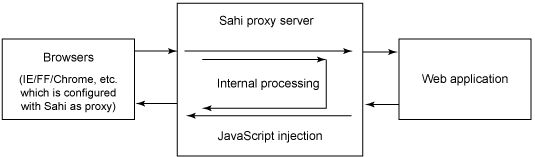
\includegraphics[width=9cm]{figures/sahi.PNG}\hspace*{\fill}
 \caption{Simulated user operation}
 \label{fig}
\end{figure}

\subsection{Telerik}
Telerik Test Studio\footnote{http://www.telerik.com/teststudio} is commercial windows-based software testing tool with Visual Studio plugins. It facilitates web and desktop (GUI) functional testing, performance testing and mobile app testing with Record and Replay features. It supports JavaScript, HTML, ASP.NET, Ajax, Silverlight etc and facilitates quick validations. It works on Internet Explorer, Firefox, Chrome and Safari. It has features like visual storyboard and 3D element selection. It also offers script-lesstest automation for Silverlight applications.Test Studio offers three product versions:\\
1. The Functional version performs web and WPF testing and includes the Visual Studio plugin.\\
2. The Load version performs load testing.\\
3. The Ultimate version combines Web, Mobile, WPF, Load testing and Test Studio for APIs.\\

\subsection{Selenium IDE}
Selenium IDE\footnote{http://www.seleniumhq.org/projects/ide/}: Selenium is known as umbrella project that enables web browser testing for all browsers. It is a open source free application supports GUI Testing and web functional testing. It is implemented as a Firefox extension, and allows recording, editing, and debugging tests. It includes the entire Selenium Core which allows easy and quick record and play back tests in the actual environment that they will run in. It supports both Windows and Linux platforms.Selenium IDE supports autocomplete mode when creating tests. This feature serves two purposes:\\
$\bullet$ It helps the tester to enter commands more quickly.\\
$\bullet$ It restricts the user from entering invalid commands.\\

\section{Evaluation of Existing Tools}
 The four tools discussed in previous section are installed on an HP laptop with Intel core i5 processor (2.30 GHz), 4 GB RAM and windows 8.1 operating system with Java 1.8. We installed the tools Sahi, Telerik and Selenium. The code for Reanimator was directly deployed on a web server we manage. Initially, to test these tools (except for Reanimator) a simple online calculator written in Javascript is deployed at 1.eecs493.pollack.tech/index1.html. Reanimator demo comes with a tile game. We used the same tile game to test Reanimator which is available at 1.eecs493.pollack.tech.\\
The following criteria are used to establish comparison between these tools:\\ \\
\textbf{ \textit{Evaluation for ease of deployment:}}
\begin{enumerate}
\item Easy to install
\item Time required to install
\item User interface
\item Tutorials available
\item Open source
\item Programming skills required
\item Documentation provided
\item Examples provided
\item User interface for developers\\
\end{enumerate}
\textbf{\textit{Evalution for level of detail of measurements:}}
\begin{enumerate}
\item Interaction with text fields
\item Mouse movements
\item Mouse clicks
\item Mouse drags
\item Scrolling
\item Dialog box\\
\end{enumerate}
\textbf{\textit{Additional system information:}}
\begin{enumerate}
\item Size
\item Platforms
\item Browser support
\item Additional features\\
\end{enumerate}

The modified version of Reanimator is deployed at 2.eecs493.pollack.tech. The developer can select the recorded session to be played from drop down list available.
Table 1 shows the comparison between Reanimator, Sahi, Telerik  and Selenium based on criteria for evalution for ease of deployment.Table 2 shows the comparison  based on criteria for evalution for level of detail of measurements.Table 3 shows the additiona system information provided with each tool. The symbol \ding{51} means that the tool provides the characteristic which is in evaluation and the symbol \ding{55} means that it doesn’t support it. \\

%\begin{wraptable}{r}{6.5cm}
\begin{figure}[h!]
 \hfill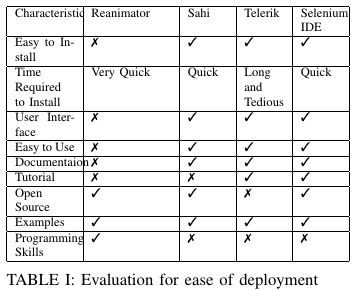
\includegraphics[width=9cm]{figures/table1.PNG}\hspace*{\fill}
\end{figure}
\begin{figure}[h!]
 \hfill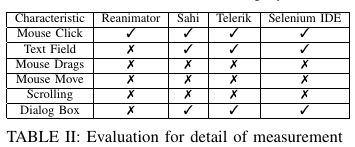
\includegraphics[width=9cm]{figures/table2.PNG}\hspace*{\fill}
\end{figure}

\begin{figure}[h!]
 \hfill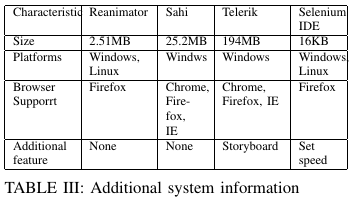
\includegraphics[width=9cm]{figures/table3.PNG}\hspace*{\fill}
\end{figure}


\section{Comparison Analysis}
The tools used here does their work of capturing and replaying the interactive sessions. But while taking other criteria into consideration, Sahi performs better than the other tools. Compared to Telerik and Reanimator, Sahi has easier installation. It has strong documentation available online. It does not require any programming skill to use Sahi. Sahi supports Chrome, Firefox and Internet Explorer. Selenium is easiest to install as it comes as firefox plugin. It also provides all the features like Sahi but the greatest setback of selenium is that it can only be used to capture and replay Firefox sessions. It has a great feature that allows the user to set speed to analyse the scenarios. No other tool provides this feature and has their own replay speed. This makes the process of analysis cumbersome if the default speed is very fast or slow. Telerik has a major setback that its installation takes very long (it took us 1 day to install) to finish since it requires lot of dependencies and also its installation process is not very effective. It requires large hard disk space. It has the feature called visual storyboard which gives the snapshot of each scenario recorded by tool. This allows the developer to go to any snapshot. We used the one month free trial version of Telerik and requires to purchase once the trial period expires. Telerik also supports Chrome, Firefox and Internet Explorer. Reanimator is a small capture and replay tool inspired by Mugshot. It requires programming skills since it does not come as ready to use testing tool. It is built on JQuery 1.8.3. It requires programming skills to get Reanimator working.Also it works only on Firefox and Internet Explorer. It does not have any additional feauture. \\
We modified Reanimator by upgrading it to JQuery 3.2.0 and enabled it to work on Chrome too. It could be seen that the old version of Reanimator provided by the developers which is available at 1.eecs493.pollack.tech does not work on Chrome. While the modified version does work on Chrome. Reanimator comes with a demo which is a tile game. We have used the same game to test the modified version.
 Based on the evalution criteria seen in table 1, 2 and 3, we choose Sahi as the best tool among all others.


\section{Extension and Modification of Reanimator}
We forked the original Reanimator GitHub project at https://github.com/brianmpollack/reanimator. It took awhile to determine exactly how the original authors built Reanimator, but we were able to understand their work update their code to work with JQuery 3.2.0, the current version.

While updating the Reanimator code, we learned why it did not initially work in Google Chrome. It appears that the original authors tried to convert DOM objects to JSON. It is commonly known that JSON does not support circular references, but DOM objects contain numerous circular references. Some browsers, such as Firefox, will simply proceed with the JSON encoding and dropped the circular references, but other browsers, such as Chrome, will terminate the JavaScript process. We found a simple function that will remove the circular references from the DOM object and convert it to JSON, allowing Reanimator to now be used in any major browser. It needs testing on browsers such as Internet Explorer and Edge, but it worked in our preliminary tests with Firefox, Chrome, and Safari.

We also found a file error in the included demos. The original Makefile added a symbolic link to link the Reanimator JavaScript code to the demos, but the symbolic link caused issues both when all the code is uploaded to GitHub and even locally on my computer. For now, we simply copied the correct files into position on our web server, but we plan to update the Makefile to copy the files automatically. We are saving this for the end of the project because we anticipate having many changes to make to the demos (to reflect our new features/code), so we will update the demos all at once.


\section{Conclusion}
In our study, we compared four capture and replay tools, namely Reanimator, Sahi, Telerik and Selenium. The goal of this study was to determine the best tool among these which has best overall performance. These tools were compared on different criteria to find out which tool has reliable capture and replay capabilities without requiring too much human efforts. After evaluating each one of the tools, we came to a conclusion that the tool that best satisfies our requirements is Sahi. This tool stood out from rest of the tools as it has best overall performance. Therefore, we can say that Sahi can be easily adapted by any developer to test their GUI application. We also worked on Reanimator to enhance it by additing new functionalities to it. We enabled it to work on Chrome. We ...{to be added by Brian}



%\bibliographystyle{IEEEtran}


\printbibliography

\end{document}
